\documentclass[journal]{new-aiaa}

\usepackage[utf8]{inputenc}
\usepackage{graphicx}
\usepackage{amsmath}
\usepackage{longtable}
\usepackage{tikz}
\usetikzlibrary{positioning,arrows.meta,fit,backgrounds,calc}
\setlength\LTleft{0pt}

\title{Scene-Adaptive Detector Operating-Point Control for Unmanned Aerial Vehicle Multi-Object Tracking}

\author{Ahmed Gouda}
\affil{Affiliation, City, Country}

\begin{document}

\maketitle

\begin{abstract}
Multi-object tracking from unmanned aerial vehicles must cope with scenes that change in density, object scale, illumination, and sharpness while running within a fixed compute budget. This paper studies causal, training-free control of the detector operating point, namely the confidence threshold, the overlap threshold of non-maximum suppression, and the input resolution, driven by a scene complexity index that combines five inexpensive image and detection cues ranked against a label-free calibration set. The controller updates every ten frames and has eleven parameters, all selected on validation data and frozen before a locked held-out test. On seventeen held-out aerial sequences, the selected controller raised higher order tracking accuracy from 28.43 to 33.84 percent over a static default while processing 38.98 decoded frames per second on one Tesla T4 graphics processor, and it transferred to a second aerial benchmark without retuning (24.08 to 28.39 percent). A matched static configuration evaluated afterwards reached 33.93 percent, so the gain comes from the validation-calibrated operating point rather than from frame-to-frame switching. The paper reports this attribution and the evidence that bounds when switching can help.
\end{abstract}

\section*{Nomenclature}

{\renewcommand\arraystretch{1.0}
\noindent\begin{longtable}{@{}l @{\quad=\quad} l@{}}
$c_t$ & detector confidence threshold applied at frame $t$ \\
$c_{\mathrm{e}}, c_{\mathrm{h}}$ & confidence threshold at $S=0$ (easy end) and at $S=1$ (hard end) \\
$\hat F_k$ & empirical distribution function of cue $k$ on the calibration set \\
$K$ & analysis stride, frames between two cue analyses \\
$N_{t}$ & number of detections kept by the controller-set confidence filter at frame $t$ \\
$q_k$ & normalized value of scene cue $k \in \{\mathrm{crowd}, \mathrm{tiny}, \mathrm{edge}, \mathrm{light}, \mathrm{blur}\}$ \\
$r_t$ & detector input resolution at frame $t$, pixels \\
$r_0, r_1, r_2$ & low, intermediate, and high resolution levels, pixels \\
$S_t$ & smoothed scene complexity index at frame $t$ \\
$s_j$ & raw scene complexity index of analysis $j$ \\
$W$ & smoothing window, number of analyses averaged \\
$w_k$ & normalized weight of cue $k$ \\
$\beta$ & mean gray level of the analysis image \\
$\eta_t$ & overlap (intersection over union) threshold of non-maximum suppression at frame $t$ \\
$\eta_{\mathrm{e}}, \eta_{\mathrm{h}}$ & suppression threshold at $S=0$ and at $S=1$ \\
$\theta_t$ & detector operating point $(c_t, \eta_t, r_t)$ \\
$\tau_{\mathrm{m}}, \tau_{\mathrm{h}}$ & complexity thresholds that switch resolution to $r_1$ and to $r_2$ \\
$\nu$ & variance of the Laplacian of the analysis image \\
$\gamma$ & mean Sobel gradient magnitude of the analysis image \\
$\Delta$ & paired difference between two systems, percentage points \\
\end{longtable}}
\addtocounter{table}{-1}

\section{Introduction}
\lettrine{C}{ameras} carried by small unmanned aerial vehicles are now routine sensors for traffic monitoring, inspection, search, and surveillance, and most of these missions need more than detection: they need persistent identities for the objects in view. Tracking by detection is the dominant way to obtain those identities in real time: a detector proposes boxes in each frame and an online tracker associates them over time \cite{bewley2016sort,wojke2017deepsort,zhang2022bytetrack}. Aerial video is a difficult case for this pipeline. Objects are small and numerous, the platform moves, and the scene changes within a single flight from sparse rural roads to dense intersections, from daylight to dusk, and from sharp to motion-blurred frames \cite{zhu2022visdrone,du2018uavdt,wu2022uavsurvey}. The same airborne perception problem appears throughout the aerospace information systems literature, from ground-target tracking by multirotor platforms \cite{miller2015multitarget} and compact descriptors for moving-object tracking \cite{desai2017uavfeature} to deep detectors deployed on board \cite{choi2022docking,lu2024uavdetection} and simulated imagery for vision-based refueling \cite{parsons2019refueling}.

A detector deployed in such a pipeline is configured by a small number of operating-point parameters: the confidence threshold that decides which boxes are passed to the tracker, the overlap threshold of non-maximum suppression (NMS), and the input resolution. They are usually set once, often to library defaults, and left unchanged. That choice has two costs. First, the defaults were chosen for generic ground-level benchmarks, not for aerial footage with many objects of a few pixels. Second, a fixed setting cannot follow the scene: a threshold that suppresses clutter in a crowded intersection may discard the few visible vehicles on an empty road, and the resolution needed to see small objects is wasted on frames that contain none. Resolution also dominates the compute budget, which matters on a platform with a fixed processor and a hard frame rate.

This paper studies whether a lightweight, causal controller that reads the scene and adjusts the detector operating point on the fly improves aerial multi-object tracking at a real-time processing rate. The controller combines five inexpensive cues, namely detection density, the fraction of tiny objects, image edge strength, low light, and blur, into a scalar scene complexity index (SCI) and maps that index to the three operating-point parameters. It learns nothing at run time, needs no labelled calibration beyond a small validation set, and adds negligible computation.

The contribution of the paper is the design, a validation-only selection protocol, and a locked held-out evaluation of this controller, together with an attribution analysis that determines where the measured gain comes from. The specific contributions are as follows:
\begin{enumerate}
\item A training-free scene-adaptive controller whose cues are ranked against a label-free calibration set derived from fixed detector outputs, so that the cue scale does not depend on ground truth or on the test data (Sec.~\ref{sec:method}).
\item A validation-only selection chain: one-at-a-time operating-point sweeps, a temporal ablation of the update schedule, a joint Bayesian-style search of cue weights and mappings under a throughput gate and an identity-switch constraint, and a multi-objective variant with a predeclared selection rule (Secs.~\ref{sec:sci}--\ref{sec:setup}).
\item A locked held-out comparison on the VisDrone2019 multi-object tracking test-dev split and a zero-tuning cross-dataset test on UAVDT, with paired sequence-level bootstrap intervals (Sec.~\ref{sec:results}).
\item An attribution analysis showing that the validation-optimized controller performs like its own matched static operating point, together with ablation evidence on when scene-driven switching does and does not add accuracy (Secs.~\ref{sec:results}--\ref{sec:failure}).
\end{enumerate}

The last point shapes the reading of the paper. The optimized controller improves substantially over the static default and over a hand-designed controller, and it generalizes to a second aerial dataset without retuning. However, a matched static configuration, evaluated after the freeze for attribution, reaches the same held-out accuracy. The gain is therefore produced by the validation-calibrated operating point and tracker profile, while switching itself contributes no measurable accuracy for this detector and this operating range. The paper reports that result as it is, explains why the optimization converged to near-static behavior, and uses the hand-designed controller's ablation to show the regime in which scene-driven resolution switching does pay off.

The remainder of the paper is organized as follows. Section~\ref{sec:related} reviews related work. Section~\ref{sec:problem} formulates the control problem. Section~\ref{sec:method} describes the cues and the index, Sec.~\ref{sec:sci} analyzes the index, Sec.~\ref{sec:control} gives the control laws, and Sec.~\ref{sec:pipeline} describes the detection and tracking pipeline. Section~\ref{sec:setup} gives the experimental protocol, Sec.~\ref{sec:results} the held-out results, Sec.~\ref{sec:ablation} the ablations, Sec.~\ref{sec:runtime} the accuracy--runtime analysis, and Sec.~\ref{sec:failure} the failure analysis. Section~\ref{sec:limits} states the limitations and Sec.~\ref{sec:conclusions} concludes.

\section{Related Work}\label{sec:related}

\subsection{Aerial detection and tracking}
The VisDrone benchmark \cite{zhu2022visdrone} and the UAVDT benchmark \cite{du2018uavdt} established large annotated drone video collections for detection and multi-object tracking, and they document the characteristic difficulties of the domain: small objects, high density, changing altitude and viewpoint, and illumination changes. Surveys of deep learning for drone-based detection and tracking \cite{wu2022uavsurvey} and of computer vision for unmanned aerial vehicles \cite{kanellakis2017uavvision} summarize the resulting methods. Methods specialized for moving aerial platforms model camera motion explicitly \cite{liu2022uavmot}, and the aerospace literature has studied airborne target tracking with explicit motion models \cite{miller2015multitarget}, efficient feature descriptors for ground moving-object tracking from small aircraft \cite{desai2017uavfeature}, onboard deep detection for real-time urban object detection \cite{lu2024uavdetection}, and onboard vision-based deep learning for docking \cite{choi2022docking}. Small-object detection, the central difficulty of aerial footage, is surveyed in \cite{cheng2023smallobject}; multi-scale feature pyramids \cite{lin2017fpn} are the standard architectural response, and input resolution remains the simplest operational lever.

\subsection{Tracking by detection}
Online trackers of the SORT family combine a constant-velocity Kalman filter \cite{kalman1960} with Hungarian assignment \cite{kuhn1955hungarian} on box overlap \cite{bewley2016sort}; DeepSORT adds appearance features \cite{wojke2017deepsort}; the IOU tracker shows how far pure overlap association can go at high frame rates \cite{bochinski2017iou}. ByteTrack associates high-confidence detections first and then recovers occluded objects from low-confidence detections \cite{zhang2022bytetrack}, and observation-centric and appearance-augmented variants refine the motion model and the association cost \cite{cao2023ocsort,maggiolino2023deepocsort,aharon2022botsort,du2023strongsort}. Joint detection and embedding \cite{zhang2021fairmot} and transformer-based end-to-end trackers \cite{zeng2022motr} remove the separate association step. Nearly all of these methods take the detector's operating point as given and tune their own thresholds against it, which is why the detector operating point and the tracker profile are treated together in this paper.

\subsection{Detector operating points}
Single-stage detectors \cite{redmon2016yolo} and two-stage detectors \cite{ren2017fasterrcnn} both expose a confidence threshold and a suppression threshold; soft suppression \cite{bodla2017softnms} replaces the hard overlap cut with score decay. The confidence scale itself is not calibrated across conditions \cite{kuppers2020detcalib}, which motivates ranking scene statistics against a reference distribution rather than using raw thresholds. In this study all operating-point parameters are selected on validation data only, with the tree-structured Parzen estimator of the Optuna framework \cite{akiba2019optuna} used as the search engine.

\subsection{Content-adaptive inference}
Adapting inference to content is an established idea. Dynamic neural networks adapt their depth, width, or resolution to the input \cite{han2022dynamic}; video analytics systems adapt configurations such as resolution and frame rate to the content and to the available resources \cite{jiang2018chameleon}; and approximate detection frameworks trade accuracy for latency according to content and contention \cite{xu2020approxdet}. These systems either learn the adaptation policy or profile many configurations online. The controller studied here is deliberately simpler: it is training-free, causal, reads five scalar cues, and changes only three detector parameters, so that its behavior can be audited and its benefit attributed.

\subsection{Evaluation}
Tracking accuracy is reported with the CLEAR multi-object tracking accuracy (MOTA) \cite{bernardin2008clear}, the identity F1 score (IDF1) \cite{ristani2016idf1}, and the higher order tracking accuracy (HOTA) \cite{luiten2021hota}, which balances detection and association, following the MOTChallenge practice \cite{dendorfer2021motchallenge}. Uncertainty is quantified by a paired bootstrap over sequences \cite{efron1993bootstrap}.

\section{Problem Formulation}\label{sec:problem}
Let $I_1, I_2, \ldots$ be the frames of a video. A detector $D$ applied to frame $I_t$ with operating point $\theta_t=(c_t,\eta_t,r_t)$ returns a set of boxes with confidence scores: the image is resized so that its long side equals $r_t$ pixels, candidate boxes are produced, boxes overlapping a higher-scoring box by more than $\eta_t$ are suppressed, and boxes with score below $c_t$ are discarded. An online tracker $T$ consumes the kept boxes and outputs identified tracks. A controller $\pi$ chooses the operating point,
\begin{equation}
\theta_t = \pi\left(I_{1:t}, \mathcal{D}_{1:t-1}\right), \qquad \theta_t \in \Theta = \mathcal{C} \times \mathcal{H} \times \mathcal{R},
\label{eq:policy}
\end{equation}
where $\mathcal{D}_{1:t-1}$ are the detections of earlier frames and $\mathcal{C}$, $\mathcal{H}$, $\mathcal{R}$ are the admissible sets of confidence thresholds, suppression thresholds, and resolutions. Equation~\eqref{eq:policy} makes the controller causal: it may use the current image and past detections but no future frame and no ground truth.

The design objective is to maximize tracking accuracy on held-out sequences subject to a processing-throughput constraint and without increasing identity fragmentation:
\begin{equation}
\max_{\pi}\; \mathrm{Acc}(\pi) \quad \text{s.t.} \quad \mathrm{FPS}(\pi) \ge 25, \qquad \mathrm{IDS}(\pi) \le \mathrm{IDS}_{\mathrm{ref}},
\label{eq:objective}
\end{equation}
where FPS is the number of processed frames per second and IDS the number of identity switches. The accuracy term and the reference are made concrete in Sec.~\ref{sec:setup}: MOTA was the selection objective, HOTA is the primary reporting metric, and $\mathrm{IDS}_{\mathrm{ref}}$ is the identity-switch count of the hand-designed controller on validation. Because held-out accuracy cannot be observed during design, Eq.~\eqref{eq:objective} is solved on a validation split, and the held-out test measures how well that solution transfers.

Three restrictions define the scope. The controller is training-free: it has no learned weights, only a small number of scalar parameters selected on validation data. The detector and the tracker are fixed and pretrained; neither is fine-tuned on aerial data. The admissible sets are finite and are themselves derived from validation sweeps (Sec.~\ref{sec:setup}), so that the controller only chooses among operating points with measured validation support.

\section{Methodology}\label{sec:method}

Figure~\ref{fig:system} shows the pipeline. Every $K$ frames, the controller computes five cues from a quarter-scale grayscale copy of the current frame and from the detections of the previous frame, ranks them against a calibration set, combines them into the raw index $s_j$, smooths the index over the last $W$ analyses, and maps the smoothed index $S_t$ to the operating point used until the next analysis.

\begin{figure}[t]
\centering
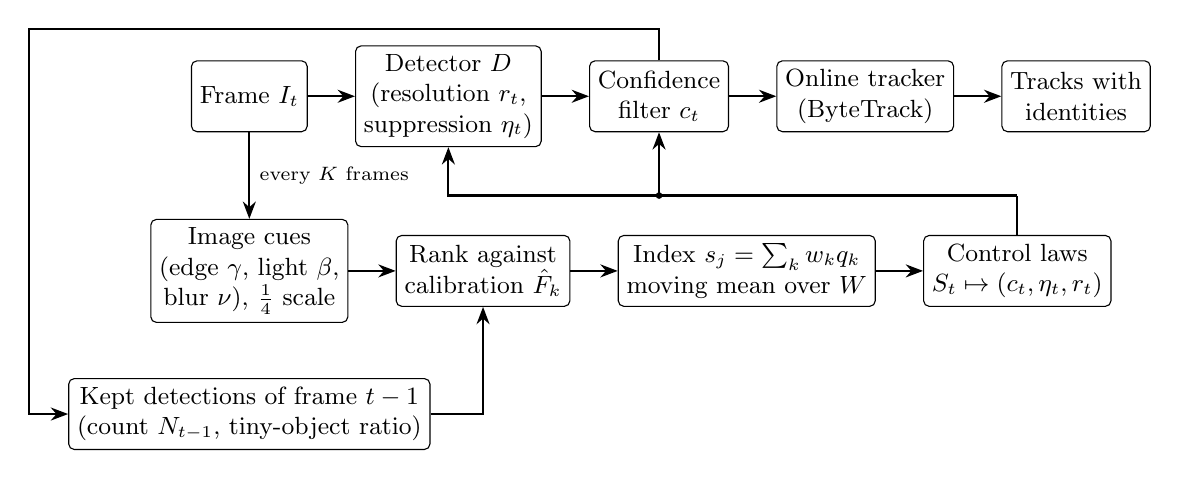
\begin{tikzpicture}[
  node distance=5mm and 6mm,
  box/.style={draw, rounded corners=2pt, align=center, font=\small, minimum height=9mm, inner sep=3pt},
  arr/.style={-{Stealth[length=2.2mm]}, thick}]
\node[box] (frame) {Frame $I_t$};
\node[box, right=of frame] (det) {Detector $D$\\(resolution $r_t$,\\suppression $\eta_t$)};
\node[box, right=of det] (conf) {Confidence\\filter $c_t$};
\node[box, right=of conf] (trk) {Online tracker\\(ByteTrack)};
\node[box, right=of trk] (out) {Tracks with\\identities};
\node[box, below=11mm of frame] (cue) {Image cues\\(edge $\gamma$, light $\beta$,\\blur $\nu$), $\tfrac14$ scale};
\node[box, right=of cue] (rank) {Rank against\\calibration $\hat F_k$};
\node[box, right=of rank] (sci) {Index $s_j=\sum_k w_k q_k$\\moving mean over $W$};
\node[box, right=of sci] (map) {Control laws\\$S_t \mapsto (c_t,\eta_t,r_t)$};
\node[box, below=7mm of cue] (prev) {Kept detections of frame $t-1$\\(count $N_{t-1}$, tiny-object ratio)};
\draw[arr] (frame) -- (det);
\draw[arr] (det) -- (conf);
\draw[arr] (conf) -- (trk);
\draw[arr] (trk) -- (out);
\draw[arr] (frame) -- node[right, font=\scriptsize]{every $K$ frames} (cue);
\draw[arr] (cue) -- (rank);
\draw[arr] (rank) -- (sci);
\draw[arr] (sci) -- (map);
\coordinate (bus) at ($(map.north)+(0,5mm)$);
\draw[thick] (map.north) -- (bus);
\draw[arr] (bus) -| (det.south);
\fill (bus -| conf.south) circle (1.2pt);
\draw[arr] (bus -| conf.south) -- (conf.south);
\draw[arr] (conf.north) -- ++(0,4mm) -| ($(prev.west)+(-5mm,0)$) -- (prev.west);
\draw[arr] (prev.east) -| (rank.south);
\end{tikzpicture}
\caption{Scene-adaptive operating-point control. The controller runs every $K=10$ frames on a quarter-scale grayscale image and on the detections kept at the previous frame; the chosen operating point is held until the next analysis.}
\label{fig:system}
\end{figure}

\subsection{Scene cues}
Five cues are computed at each analysis. They were chosen because each targets a failure mode of aerial detection and each costs at most a few image passes on a quarter-resolution frame.

\emph{Crowd.} The number $N_{t-1}$ of detections kept at the previous frame measures density. It is a detector-derived quantity, not a ground-truth count.

\emph{Tiny-object ratio.} The fraction of the previous frame's kept detections whose box area is below $32\times32$ pixels,
\begin{equation}
q_{\mathrm{tiny}} = \frac{1}{N_{t-1}} \sum_{i=1}^{N_{t-1}} \mathbf{1}\left[a_i < 32^2\right],
\label{eq:tiny}
\end{equation}
with $q_{\mathrm{tiny}}=0$ when $N_{t-1}=0$, measures how much of the scene is at the scale where detectors lose recall \cite{cheng2023smallobject}.

\emph{Edge strength.} The mean Sobel gradient magnitude $\gamma$ of the quarter-scale grayscale image measures texture and clutter.

\emph{Low light.} The mean gray level $\beta$ of the same image measures illumination.

\emph{Blur.} The variance $\nu$ of the Laplacian of the same image is a standard focus measure \cite{pechpacheco2000blur}; low values indicate blur.

\subsection{Label-free calibration}
Raw cue values have incomparable units and dataset-dependent ranges. Each cue is therefore mapped to $[0,1]$ by its empirical distribution function on a calibration set,
\begin{equation}
\hat F_k(x) = \frac{1}{M} \left|\{ m : x_m^{(k)} \le x \}\right|,
\label{eq:rank}
\end{equation}
where $x_m^{(k)}$, $m=1,\ldots,M$, are the calibration values of cue $k$. The normalized cues are
\begin{equation}
q_{\mathrm{crowd}}=\hat F_{N}(N_{t-1}),\quad q_{\mathrm{edge}}=\hat F_{\gamma}(\gamma),\quad q_{\mathrm{light}}=1-\hat F_{\beta}(\beta),\quad q_{\mathrm{blur}}=1-\hat F_{\nu}(\nu),
\label{eq:cues}
\end{equation}
and $q_{\mathrm{tiny}}$ is already a fraction. The calibration set contains $M=288$ analysis samples taken every ten frames from the seven VisDrone validation sequences, with image statistics from the frames and crowd counts from the fixed detector run at a single anchor operating point (960 pixels, confidence 0.35, suppression threshold 0.35; person, car, bus, and truck classes). No ground-truth count enters the calibration. On this set the median gray level is 107.6 (interquartile range 85.4--185.1), the median Laplacian variance is 1980, the median gradient magnitude is 66.2, and the median detection count is 10.5 (maximum 41).

The ranking makes the index invariant to monotone rescaling of each cue, and it makes the weights interpretable: a weight multiplies a quantile, not a unit-dependent value. It also means that the index describes a scene relative to the calibration distribution, so that a scene is "complex" if it is more cluttered, darker, blurrier, denser, or has more tiny objects than typical validation scenes.

\subsection{Scene complexity index}
The raw index of analysis $j$ is a convex combination of the normalized cues,
\begin{equation}
s_j = \mathrm{clip}\left(\sum_{k} w_k q_k,\, 0,\, 1\right), \qquad w_k \ge 0,\quad \sum_k w_k = 1,
\label{eq:sci}
\end{equation}
and the smoothed index is the mean of the last $W$ raw values,
\begin{equation}
S_t = \frac{1}{\min(j,W)} \sum_{i=\max(1,j-W+1)}^{j} s_i, \qquad t \in [\,1+(j-1)K,\; jK\,].
\label{eq:smooth}
\end{equation}
Analyses occur at frames $t=1, 1+K, 1+2K, \ldots$; between analyses the index and the operating point are held. With $K=10$ and $W=7$, the index at 30 frames per second reflects roughly the last two seconds and changes at most three times per second. The controller state is reset at the start of each sequence.

\section{Scene Complexity Index Analysis}\label{sec:sci}

\subsection{Frozen weights}
Figure~\ref{fig:sci}a shows the normalized weights of the two frozen profiles, the quality profile Q (trial 24 of the single-objective search) and the balanced profile B (trial 22 of the multi-objective search). Both place the largest weight on edge strength (0.434 for Q and 0.508 for B), a second tier on the tiny-object ratio (0.222 and 0.175) and on crowd density (0.129 and 0.165), and small weights on low light and blur (0.054 and 0.161 for Q; 0.121 and 0.032 for B). The weight on edge strength agrees with the intuition that textured urban scenes are the hard ones for aerial detection. The two searches disagree on blur and low light, which suggests that those cues are weakly identified by seven validation sequences.

\begin{figure}[t]
\centering
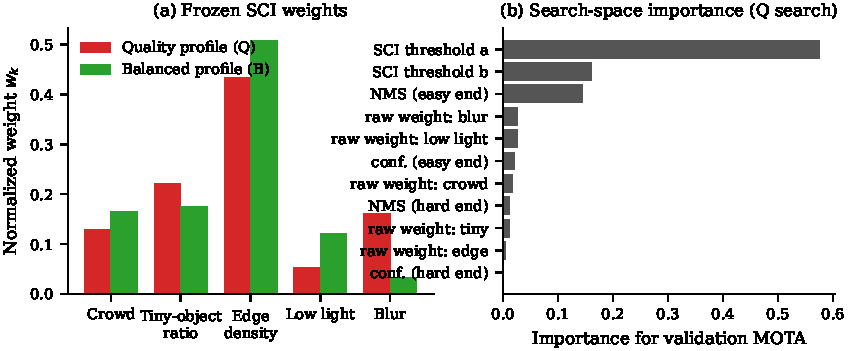
\includegraphics[width=0.95\textwidth]{figures/fig2_sci_composition.pdf}
\caption{Composition of the scene complexity index. (a) Normalized cue weights of the frozen quality profile Q and balanced profile B. (b) Importance of each search parameter for validation MOTA in the single-objective search that produced Q, as stored with the search record; the two index thresholds dominate.}
\label{fig:sci}
\end{figure}

\subsection{What the search actually tuned}
The parameter importance scores stored with the single-objective search (Fig.~\ref{fig:sci}b) are more revealing than the weights. The two thresholds of the resolution rule account for most of the explained variation in validation MOTA (0.575 and 0.161), followed by the easy-end suppression threshold (0.145); every cue weight has importance below 0.03. In other words, the search mostly tuned \emph{how often the controller uses high resolution}, not how the scene is described. The frozen thresholds of Q ($\tau_{\mathrm{m}}=0.135$, $\tau_{\mathrm{h}}=0.287$) are low relative to the typical index, so Q runs at 960 pixels on almost every frame: its mean resolution is 957 pixels on validation and 955 pixels on UAVDT. Its suppression threshold is constant ($\eta_{\mathrm{e}}=\eta_{\mathrm{h}}=0.35$), and only its confidence threshold moves, between 0.30 and 0.40, with a validation mean of 0.341. The optimized quality controller is therefore close to a static operating point at (960, 0.34, 0.35). This observation is the key to the attribution result of Sec.~\ref{sec:results}.

The balanced profile behaves differently. Its thresholds ($\tau_{\mathrm{m}}=0.293$, $\tau_{\mathrm{h}}=0.666$) place typical scenes in the intermediate and high levels and simple scenes at 512 pixels, giving mean resolutions of 825 pixels on validation, 869 pixels on test-dev, and 829 pixels on UAVDT. Its confidence threshold is constant at 0.40, and its suppression threshold tightens from 0.60 in simple scenes to 0.35 in complex ones (mean 0.47--0.50). Profile B is thus the one that actually switches, and it trades accuracy for fewer identity switches, fewer false positives, and higher throughput.

\subsection{Feedback through the crowd cue}
The crowd and tiny-object cues are computed from detections that already passed the controller's own confidence filter, which closes a loop. In Q the confidence threshold rises with the index; a higher index therefore removes low-scoring boxes, lowers the next crowd count, and pulls the index back down. This is negative feedback, which keeps the operating point stable. The hand-designed controller of Sec.~\ref{sec:control} lowers the confidence threshold as the index rises, which admits more boxes and raises the next crowd count: positive feedback, bounded only by the clipping of its thresholds. The moving mean of Eq.~\eqref{eq:smooth} and the ten-frame stride damp both loops. The analysis does not change any result, but it explains why the validation search preferred a controller whose confidence threshold increases with complexity.

\section{Adaptive Control Strategy}\label{sec:control}

\subsection{Calibrated control laws}
The calibrated controller maps the smoothed index to the operating point by two linear laws and one piecewise-constant law:
\begin{align}
c_t &= c_{\mathrm{e}} + S_t\,(c_{\mathrm{h}} - c_{\mathrm{e}}), \label{eq:conf}\\
\eta_t &= \eta_{\mathrm{e}} + S_t\,(\eta_{\mathrm{h}} - \eta_{\mathrm{e}}), \label{eq:nms}\\
r_t &= \begin{cases} r_0, & S_t < \tau_{\mathrm{m}},\\ r_1, & \tau_{\mathrm{m}} \le S_t < \tau_{\mathrm{h}},\\ r_2, & S_t \ge \tau_{\mathrm{h}}, \end{cases} \label{eq:res}
\end{align}
with resolution levels $(r_0, r_1, r_2) = (512, 928, 960)$ pixels. The eleven parameters are the five weights, the four endpoints $c_{\mathrm{e}}, c_{\mathrm{h}}, \eta_{\mathrm{e}}, \eta_{\mathrm{h}}$, and the two thresholds $\tau_{\mathrm{m}}, \tau_{\mathrm{h}}$. Figure~\ref{fig:map} plots the three laws for both profiles, and Table~\ref{tab:settings} lists all frozen configurations.

\begin{figure}[t]
\centering
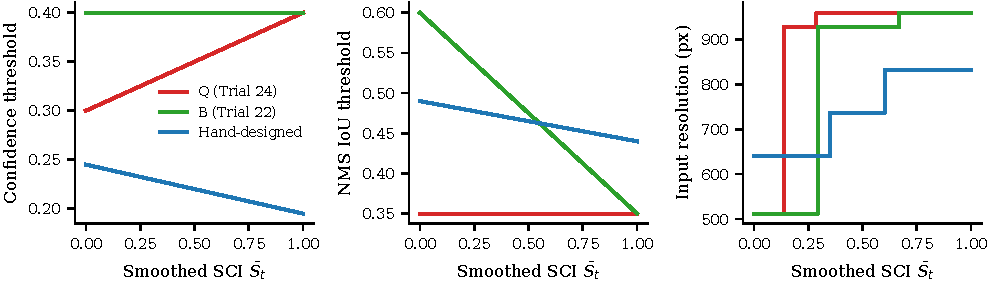
\includegraphics[width=0.95\textwidth]{figures/fig3_adaptation_map.pdf}
\caption{Adaptation maps: confidence threshold, suppression threshold, and input resolution as functions of the smoothed index for the quality profile Q, the balanced profile B, and the hand-designed controller (scene-label adjustments of the hand-designed controller omitted).}
\label{fig:map}
\end{figure}

\begin{table}[t]
\centering
\caption{Frozen configurations compared in this study. Confidence and NMS entries give the value at $S=0$ and at $S=1$ (linear in between); resolution is the long-side input size in pixels. All adaptive controllers analyze every $K=10$ frames with a moving mean over $W=7$ analyses.}
\label{tab:settings}
\small
\begin{tabular}{p{3.3cm}p{3.0cm}p{3.0cm}p{3.8cm}p{1.2cm}}
\hline
Configuration & Confidence & NMS IoU & Resolution & Tracker \\
\hline
Static default & 0.25 & 0.45 & 640 & default \\
Hand-designed controller & $0.245-0.05S$, clipped to 0.19--0.28 & $0.49-0.05S$, clipped to 0.40--0.52 & 640/736/832 (rules in Sec.~\ref{sec:control}) & tuned \\
Quality profile Q (trial 24) & 0.30$\to$0.40 & 0.35$\to$0.35 & 512/928/960 at $S\ge0.135/0.287$ & tuned \\
Balanced profile B (trial 22) & 0.40$\to$0.40 & 0.60$\to$0.35 & 512/928/960 at $S\ge0.293/0.666$ & tuned \\
Matched static anchor & 0.35 & 0.35 & 960 & tuned \\
\hline
\multicolumn{5}{l}{Tracker profiles (ByteTrack): default = high 0.25, low 0.10, new 0.25, buffer 30, match 0.80;}\\
\multicolumn{5}{l}{tuned = high 0.18, low 0.04, new 0.20, buffer 45, match 0.86.}\\
\hline
\end{tabular}
\end{table}


\subsection{Hand-designed controller}
The hand-designed controller is the earlier version of the same idea and serves as the adaptive baseline. Its index uses fixed saturating transforms instead of calibrated ranks:
\begin{equation}
s_j = \mathrm{clip}\left(0.30\min\left(\tfrac{N_{t-1}}{30},1\right) + 0.20\min\left(\tfrac{e}{0.14},1\right) + 0.30\,q_{\mathrm{tiny}} + 0.10\,\mathbf{1}[\beta<80] + 0.05\,\mathbf{1}[\nu<180],\;0,\;1\right),
\label{eq:heur}
\end{equation}
where $e$ is the fraction of Canny edge pixels of the quarter-scale image. It also assigns a scene label (night, blur, tiny, crowded, or clear) from the same cues. Its confidence threshold $0.245-0.05S_t$ decreases with complexity, is lowered by a further 0.012 in crowded, tiny, or night scenes, and is clipped to $[0.19, 0.28]$; its suppression threshold $0.49-0.05S_t$ is lowered by 0.012 in blurred scenes and clipped to $[0.40, 0.52]$. Its resolution is 832 pixels when $S_t>0.60$ or the tiny-object ratio exceeds 0.5, 736 pixels when $S_t>0.35$ or the scene is labelled crowded or tiny, and 640 pixels otherwise. It uses the same analysis stride and smoothing window as the calibrated controller ($K=10$, $W=7$).

The two controllers encode opposite hypotheses about confidence. The hand-designed controller is recall-oriented: in hard scenes it admits weaker boxes. The calibrated profiles are precision-oriented: Q raises the confidence threshold in hard scenes, and B holds it at 0.40 while tightening suppression. The validation evidence of Sec.~\ref{sec:ablation} favors the precision-oriented choice for this detector and tracker.

\subsection{Update schedule and cost}
All controllers analyze the first frame of each sequence and every tenth frame thereafter; the image cues require one resize, one color conversion, two Sobel filters, and one Laplacian on a quarter-scale image, and the detection cues reuse boxes that the tracker already holds. In the matched static run on test-dev, where the controller code path ran without cue analysis, the per-frame controller time was 0.005 ms against 19.5 ms for the detector and 3.6 ms for the tracker. The cue analysis cost of the adaptive runs was not profiled separately; it is included in their end-to-end processing throughput.

\section{Detection and Tracking Pipeline}\label{sec:pipeline}

\subsection{Detector}
The detector is the Ultralytics YOLOv8n model pretrained on the COCO dataset (Ultralytics library version 8.3.200), run in half precision through PyTorch on one NVIDIA Tesla T4 graphics processor with at most 1000 detections per frame. Only the person, car, bus, and truck classes are kept on VisDrone; car, bus, and truck are kept on UAVDT, whose annotations cover vehicles only. The detector is not fine-tuned on aerial data, which keeps the controller evaluation independent of any training choice but also bounds the absolute accuracy (Sec.~\ref{sec:limits}).

\subsection{Tracker}
The tracker is the Ultralytics implementation of ByteTrack \cite{zhang2022bytetrack} with score fusion and a nominal frame rate of 30. Two profiles are used (Table~\ref{tab:settings}): the library-style default profile (high threshold 0.25, low threshold 0.10, new-track threshold 0.25, buffer 30 frames, matching threshold 0.80) and a tuned profile selected in earlier validation work (0.18, 0.04, 0.20, 45 frames, 0.86). The tuned profile is part of every adaptive system and of the matched static anchor; the static default uses the default profile.

One interaction between detector and tracker needs to be stated explicitly. Detections below the controller's confidence threshold are removed before the tracker. Because every confidence threshold used in this study (0.19 or higher) is at or above the tracker's high threshold, every detection reaching the tracker counts as high-confidence, and all of them except boxes of the hand-designed controller scored between 0.19 and 0.20 are eligible to start a new track. ByteTrack's second association stage, which recovers occluded objects from low-confidence boxes, therefore receives no input in these configurations. The tuned profile acts mainly through its longer buffer and its looser matching threshold.

\subsection{Timing protocol}
Throughput is reported as processing frames per second: the number of frames divided by the summed per-frame time of cue analysis, detection (with device synchronization), and tracking. Frames are decoded from JPEG files before timing, and all resolutions a system can request are warmed up before the first timed frame. Decoding is excluded because an onboard pipeline receives decoded frames from the camera. In the matched static run, decoding cost 22.5 ms per frame on average, and throughput including decoding was 21.90 frames per second, below the 25 frames-per-second target. The real-time statements of this paper therefore apply to already-decoded frames. The gate of 25 frames per second was applied to the whole-split processing throughput.

\section{Experimental Setup}\label{sec:setup}

\subsection{Data}
Table~\ref{tab:data} lists the data. All design decisions used the seven sequences of the VisDrone2019 multi-object tracking validation split \cite{zhu2022visdrone}. The seventeen sequences of the test-dev split were held out until a locked three-system comparison. The twenty sequences of the UAVDT test split \cite{du2018uavdt} were used once, as a zero-tuning cross-dataset test.

\begin{table}[t]
\centering
\caption{Data splits and their role. No test sequence was used for any selection, calibration, or tuning decision.}
\label{tab:data}
\small
\begin{tabular}{llrrl}
\hline
Dataset & Split & Sequences & Frames & Role \\
\hline
VisDrone2019-MOT & validation & 7 & 2,846 & cue calibration, sweeps, ablations, optimization \\
VisDrone2019-MOT & test-dev & 17 & 6,635 & locked held-out comparison \\
UAVDT & test & 20 & 16,592 & zero-tuning cross-dataset test \\
\hline
\end{tabular}
\end{table}


\subsection{Evaluation protocol}
Evaluation is class-agnostic. On VisDrone, ground-truth boxes of the pedestrian, car, van, truck, and bus categories are kept when they are marked as considered, with occlusion and truncation levels below 2; all detector classes are pooled. This is a research protocol, not the official VisDrone evaluation, so the absolute numbers are not comparable with the VisDrone leaderboard. On UAVDT, a frozen adapter (checked by a self-test on a training sequence, which it reproduced with perfect scores) removes ground truth marked out of scope, normalizes identities, removes predictions strictly contained in ignore regions for the eighteen sequences that provide them, and matches at an overlap of 0.5. All metrics were computed with the TrackEval library pinned to commit 12c8791.

HOTA is the primary metric because it weighs detection and association equally \cite{luiten2021hota}; MOTA, IDF1, identity switches, false negatives, and false positives are reported alongside. Uncertainty is quantified by a paired bootstrap over sequences \cite{efron1993bootstrap}: sequences are resampled with replacement 5,000 times (seed 42), the metric difference between two systems is recomputed on each resample from the pooled counts, and the 2.5th and 97.5th percentiles form the 95\% interval. A win, tie, or loss count per sequence is reported as a complementary, distribution-free summary.

\subsection{Selection chain}
The selection chain used the validation split only.

\emph{Operating-point sweeps.} With the tuned tracker, three one-at-a-time sweeps measured validation accuracy and throughput for resolutions from 512 to 960 pixels in steps of 32, confidence thresholds from 0.05 to 0.50, and suppression thresholds from 0.30 to 0.80. Confidence and suppression values were kept if they met the throughput gate and at least the reference accuracy of the sweep, which retained confidence values 0.25--0.45 and suppression values 0.30--0.70. Three resolution levels were retained by a predeclared rule: a low-compute feasible level, the highest-quality feasible level, and the highest-quality distinct intermediate level, which gave 512, 960, and 928 pixels.

\emph{Temporal settings.} A grid of smoothing windows $W\in\{1,3,5,7,9\}$ and analysis strides $K\in\{1,5,10,15,20\}$ was evaluated with the hand-designed controller, and $W=7$, $K=10$ was frozen.

\emph{Quality profile.} A tree-structured Parzen estimator search of at most 50 trials explored the five raw weights (normalized to sum to one), the confidence and suppression endpoints within the retained sets, and the two resolution thresholds. The selection rule, fixed before the search, required the throughput gate and no more identity switches than the hand-designed controller on validation (271), and then selected the highest MOTA, breaking ties by fewer identity switches, then HOTA, IDF1, and throughput. Trial 24 was selected, with validation HOTA 36.11\%, MOTA 23.04\%, IDF1 40.76\%, 270 identity switches, and 37.17 frames per second.

\emph{Balanced profile.} A second, multi-objective search (seed 42) maximized MOTA and minimized identity switches with only the throughput gate. Of 50 planned trials, 49 completed. The Pareto front ranged from trial 16 (MOTA 22.83\%, 308 switches) to trial 8 (11.54\%, 114 switches). A balanced score, declared before the search, averaged min--max normalized MOTA and normalized identity-switch reduction, and it selected trial 22 (validation MOTA 19.33\%, HOTA 31.65\%, 168 switches, 51.41 frames per second).

\subsection{Held-out protocol}
Before the test split was opened, a protocol file fixed the three compared systems (static default, hand-designed controller, quality profile Q), their configuration hashes, the calibration hash, the ground-truth filter, the evaluator commit, the throughput gate, and the requirement of a T4 processor. Each system ran as a separate worker in its own session and wrote an immutable result file; the merge step refused to run until all three existed. The quality-profile worker resumed from per-sequence checkpoints after an interruption, with no parameter change. The balanced profile was frozen after its selection and tested with the same machinery; its first test attempt was interrupted before any result was saved, and an exact technical rerun of the frozen configuration produced the reported result. The UAVDT test was run for the static default and both frozen profiles under a separate lock that forbade any tuning, recalibration, or selection on UAVDT.

After these tests were complete, the matched static anchor (960 pixels, confidence 0.35, suppression 0.35, tuned tracker, no adaptation) was evaluated on test-dev and paired with the quality profile. It was not part of the preregistered comparison: it serves only to attribute the measured gain, and its throughput was measured in a separate session.

\section{Main Results}\label{sec:results}

\subsection{Held-out test-dev}
Table~\ref{tab:main} gives the held-out results and Table~\ref{tab:boot} the paired bootstrap intervals.

\begin{table}[t]
\centering
\caption{Held-out results (percent for HOTA, MOTA, IDF1; counts for IDS, FN, FP; processing frames per second on one NVIDIA Tesla T4, each system measured in its own session). No entry is marked as best because the profiles target different trade-offs.}
\label{tab:main}
\small
\begin{tabular}{lrrrrrrr}
\hline
System & HOTA & MOTA & IDF1 & IDS & FN & FP & FPS \\
\hline
\multicolumn{8}{l}{\textit{VisDrone2019-MOT test-dev (17 sequences, 6,635 frames)}}\\
Static default & 28.43 & 19.73 & 32.72 & 1235 & 155051 & 16308 & 36.53 \\
Heuristic controller & 32.70 & 23.24 & 39.52 & 1061 & 138967 & 25025 & 41.96 \\
Quality profile Q & 33.84 & 26.95 & 41.55 & 1184 & 136858 & 19029 & 38.98 \\
Balanced profile B & 31.22 & 23.79 & 37.87 & 919 & 149307 & 13632 & 46.02 \\
Matched static anchor & 33.93 & 27.00 & 41.77 & 1197 & 136391 & 19374 & 43.23$^{a}$ \\
\multicolumn{8}{l}{\textit{UAVDT test (20 sequences, 16,592 frames), no tuning on UAVDT}}\\
Static default & 24.08 & 13.84 & 27.89 & 558 & 270189 & 22974 & 65.01 \\
Quality profile Q & 28.39 & 17.40 & 34.45 & 321 & 258376 & 22896 & 58.35 \\
Balanced profile B & 26.93 & 16.12 & 32.01 & 308 & 266894 & 18758 & 61.46 \\
\hline
\multicolumn{8}{l}{$^{a}$Run after the freeze for attribution only; frames per second measured in a separate T4 session.}\\
\hline
\end{tabular}
\end{table}


\begin{table}[t]
\centering
\caption{Paired sequence-level bootstrap (5,000 resamples, seed 42): observed difference and 95\% percentile interval. HOTA, MOTA and IDF1 in percentage points; IDS reduction in switches (positive = fewer switches for the first system).}
\label{tab:boot}
\small
\resizebox{\textwidth}{!}{%
\begin{tabular}{llllll}
\hline
Data & Comparison & $\Delta$HOTA & $\Delta$MOTA & $\Delta$IDF1 & IDS reduction \\
\hline
VisDrone & Q vs static default & +5.41 [+4.13, +6.90] & +7.22 [+5.44, +9.29] & +8.82 [+6.90, +11.05] & +51 [-114, +219] \\
VisDrone & Q vs hand-designed & +1.14 [+0.14, +2.27] & +3.71 [+2.39, +5.19] & +2.03 [+0.59, +3.77] & -123 [-244, -14] \\
VisDrone & Q vs matched static anchor & -0.09 [-0.25, +0.06] & -0.05 [-0.25, +0.16] & -0.23 [-0.50, +0.02] & +13 [-23, +46] \\
VisDrone & B vs static default & +2.79 [+0.75, +4.66] & +4.06 [+0.95, +6.89] & +5.15 [+2.03, +8.08] & +316 [+175, +470] \\
VisDrone & B vs Q & -2.62 [-4.00, -1.69] & -3.16 [-6.14, -1.35] & -3.68 [-5.88, -2.24] & +265 [+82, +502] \\
UAVDT & Q vs static default & +4.30 [+2.74, +5.71] & +3.56 [+1.45, +5.81] & +6.57 [+3.81, +8.82] & +237 [+104, +377] \\
UAVDT & B vs static default & +2.85 [+1.24, +4.35] & +2.28 [+0.72, +4.16] & +4.13 [+1.63, +6.49] & +250 [+110, +404] \\
UAVDT & B vs Q & -1.46 [-2.19, -0.91] & -1.28 [-2.44, -0.20] & -2.44 [-3.74, -1.37] & +13 [-20, +50] \\
\hline
\end{tabular}}
\end{table}


Against the static default, the quality profile raised HOTA from 28.43\% to 33.84\% ($\Delta=+5.41$, 95\% interval $[+4.13, +6.90]$), MOTA by 7.22 points, and IDF1 by 8.82 points, and it won on all 17 sequences. The gain comes mostly from recall: false negatives fell by 18,193, while false positives rose by 2,721. Identity switches fell by 51, but that interval includes zero. Throughput was 38.98 frames per second against 36.53 for the default, both above the gate.

Against the hand-designed controller, the quality profile gained 1.14 HOTA points ($[+0.14, +2.27]$), 3.71 MOTA points, and 2.03 IDF1 points, and it won on 13 of 17 sequences. It produced 5,996 fewer false positives and 2,109 fewer false negatives, but 123 more identity switches, and that difference is significant ($[-244, -14]$ in switch reduction). The hand-designed controller therefore remains the identity-switch leader of the preregistered comparison, and the quality profile is not better on every metric.

The balanced profile sits at a different point of the trade-off. On test-dev it had the fewest identity switches (919), the fewest false positives (13,632), and the highest throughput (46.02 frames per second), with HOTA 31.22\%. It was significantly better than the static default on every metric, including 316 fewer identity switches ($[+175, +470]$), and significantly worse than the quality profile in HOTA ($-2.62$), MOTA, and IDF1, while having 265 fewer switches ($[+82, +502]$).

\subsection{Cross-dataset test without tuning}
On UAVDT, no parameter was changed. The quality profile raised HOTA from 24.08\% to 28.39\% ($[+2.74, +5.71]$), MOTA by 3.56 points, and IDF1 by 6.57 points, and it reduced identity switches from 558 to 321 ($[+104, +377]$), winning 15 of 20 sequences with 2 ties and 3 losses. The balanced profile improved over the default by 2.85 HOTA points ($[+1.24, +4.35]$) with 250 fewer switches, but it was significantly below the quality profile in HOTA ($-1.46$), MOTA, and IDF1, and its 13-switch advantage over the quality profile is not significant ($[-20, +50]$). Both profiles ran slower than the static default on UAVDT (58.35 and 61.46 against 65.01 frames per second), because both use higher mean resolutions than the default's 640 pixels.

Across both datasets, the quality profile is the accuracy leader of the frozen systems, and the balanced profile is a reproducible identity, false-positive, and throughput trade-off on VisDrone whose identity advantage over the quality profile does not transfer significantly to UAVDT.

\subsection{Attribution: the matched static anchor}
The quality profile runs at the top resolution on almost every frame with a confidence threshold near 0.34 and a constant suppression threshold of 0.35 (Sec.~\ref{sec:sci}). Its natural control is therefore the static operating point (960, 0.35, 0.35) with the same tuned tracker, which is also the anchor of the cue calibration. On validation, that anchor reached 36.08\% HOTA against 36.11\% for the full quality profile (Table~\ref{tab:ablation}). On test-dev, the anchor reached 33.93\% HOTA against 33.84\% for the quality profile: $\Delta=-0.09$ for the profile, with interval $[-0.25, +0.06]$ (Table~\ref{tab:boot}). MOTA, IDF1, and identity switches likewise differ by amounts whose intervals include zero.

The held-out gains of the quality profile over the static default (+5.41 HOTA) and over the hand-designed controller (+1.14) are therefore attributable to the validation-calibrated operating point, namely high resolution, a precision-oriented confidence threshold, a tight suppression threshold, and the tuned tracker profile, and not to frame-to-frame switching. The frozen protocol and the post hoc anchor jointly support that conclusion; the anchor was not available as a preregistered competitor, which is why the paper reports it as an attribution analysis rather than as a fourth system of the locked comparison.

\subsection{Per-sequence behavior}
Figure~\ref{fig:perseq} shows the per-sequence HOTA differences. On test-dev, the gain of the quality profile over the default is positive everywhere and ranges from +1.07 to +13.10 points; the largest gain occurs on the sequence where all systems are weakest (default HOTA 7.10\%). Against the hand-designed controller, four sequences are losses, the largest by 4.69 points. On UAVDT, the gains of both profiles are positive on most sequences, with a tail of losses discussed in Sec.~\ref{sec:failure}.

\begin{figure}[t]
\centering
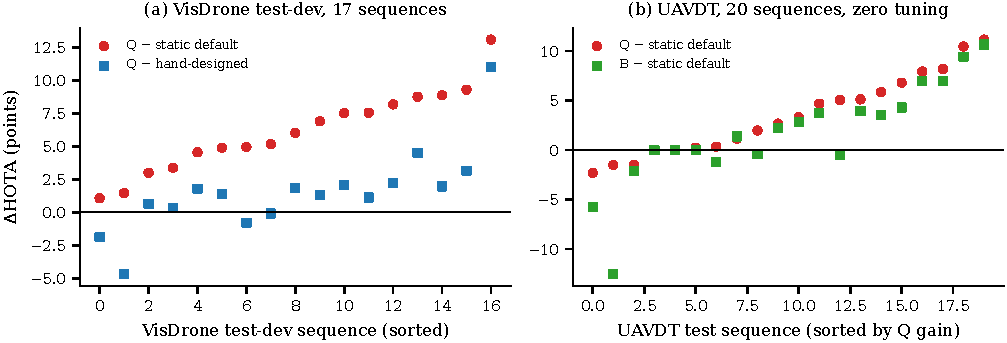
\includegraphics[width=0.95\textwidth]{figures/fig6_per_sequence.pdf}
\caption{Per-sequence HOTA differences, sorted. (a) VisDrone test-dev: quality profile minus static default and minus the hand-designed controller. (b) UAVDT: quality and balanced profiles minus static default, without any tuning on UAVDT.}
\label{fig:perseq}
\end{figure}

\section{Ablation}\label{sec:ablation}
Table~\ref{tab:ablation} and Fig.~\ref{fig:ablation} decompose both controllers on the validation split.

\begin{table}[t]
\centering
\caption{Component ablations on VisDrone2019-MOT validation (7 sequences). FPS is processing throughput on a T4; mean resolution, confidence and NMS are averaged over frames.}
\label{tab:ablation}
\small
\begin{tabular}{llrrrrrrrr}
\hline
Stage & Components & HOTA & MOTA & IDF1 & IDS & FPS & Res. & Conf. & NMS \\
\hline
\multicolumn{10}{l}{\textit{Hand-designed controller}}\\
H0 & static default, default tracker & 29.84 & 17.63 & 30.89 & 283 & 44.1 & 640 & 0.250 & 0.450 \\
H1 & + tuned tracker & 30.86 & 17.80 & 32.85 & 217 & 44.5 & 640 & 0.250 & 0.450 \\
H2 & + adaptive conf./NMS (640 px) & 31.38 & 17.64 & 33.73 & 210 & 40.7 & 640 & 0.218 & 0.474 \\
H2R & tuned tracker + adaptive resolution only & 32.45 & 18.42 & 35.67 & 241 & 39.6 & 722 & 0.250 & 0.450 \\
H3 & full hand-designed controller & 33.06 & 18.16 & 36.30 & 271 & 38.0 & 725 & 0.218 & 0.474 \\
\multicolumn{10}{l}{\textit{Optimized controller (quality profile Q)}}\\
C0 & static anchor 960/0.35/0.35, tuned tracker & 36.08 & 23.08 & 40.60 & 266 & 37.9 & 960 & 0.350 & 0.350 \\
C1 & + adaptive confidence & 36.11 & 23.01 & 40.73 & 271 & 35.3 & 960 & 0.341 & 0.350 \\
C2 & + adaptive NMS & 36.11 & 23.01 & 40.73 & 271 & 35.5 & 960 & 0.341 & 0.350 \\
C3 & + adaptive resolution (full Q) & 36.11 & 23.04 & 40.76 & 270 & 35.4 & 957 & 0.341 & 0.350 \\
\hline
\end{tabular}
\end{table}


\begin{figure}[t]
\centering
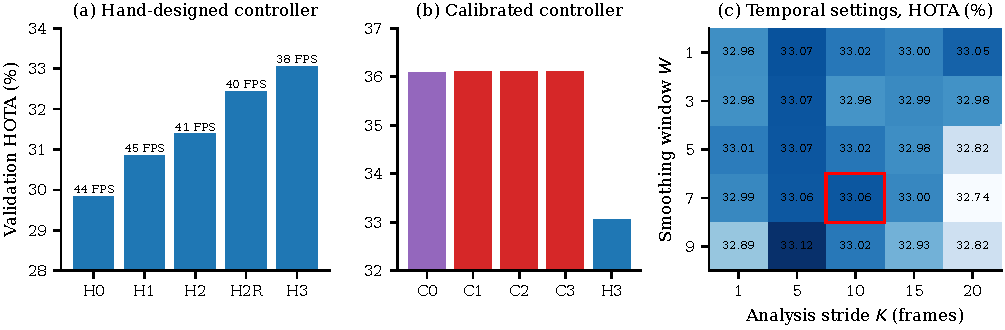
\includegraphics[width=0.95\textwidth]{figures/fig5_ablation.pdf}
\caption{Validation ablations. (a) Hand-designed controller: H0 static default with default tracker; H1 tuned tracker; H2 adaptive confidence and suppression at 640 pixels; H2R adaptive resolution only; H3 full controller. (b) Calibrated controller: C0 static anchor; C1 adaptive confidence; C2 adaptive confidence and suppression; C3 full quality profile; H3 shown for reference. (c) Temporal grid of the hand-designed controller, selected setting outlined.}
\label{fig:ablation}
\end{figure}

\subsection{Hand-designed controller}
Starting from the static default (H0, 29.84\% HOTA), tuning the tracker (H1) added 1.03 HOTA points and removed 66 identity switches at unchanged throughput. Adaptive confidence and suppression at a fixed 640 pixels (H2) added a further 0.52 points. Adaptive resolution alone, with static confidence and suppression (H2R), reached 32.45\%, 1.59 points above H1, at a mean resolution of 722 pixels. The full controller (H3) reached 33.06\%, 2.20 points above H1, at 38.0 frames per second against 44.5 for H1. For the hand-designed controller, therefore, scene-driven switching does add accuracy, and most of it comes from resolution. The operating range of that controller is narrow and low (640--832 pixels), and its adaptive resolution moves the operating point into the range where accuracy grows fastest with resolution (Table~\ref{tab:speed}).

\subsection{Calibrated controller}
For the quality profile the picture is different. The static anchor (C0) already reached 36.08\% HOTA, 3.01 points above the full hand-designed controller. Adding adaptive confidence (C1) changed HOTA by +0.03 points and identity switches by +5. Adding adaptive suppression (C2) changed nothing, as expected, because the profile's two suppression endpoints are equal; the identical metrics confirm that the ablation machinery isolates components exactly. Adding adaptive resolution (C3) changed HOTA by less than 0.01 points, because the index almost never falls below the resolution thresholds. The components of the calibrated controller are therefore measurable but negligible, which the held-out anchor comparison of Sec.~\ref{sec:results} confirms on unseen data.

\subsection{Temporal settings}
Across the 25 temporal settings, HOTA of the hand-designed controller varied only between 32.74\% and 33.12\% (Table~\ref{tab:temporal}); the frozen setting $W=7$, $K=10$ gave 33.06\%. Analyzing every frame ($K=1$) cost 6 to 14 frames per second relative to $K\ge5$ in the same grid without an accuracy benefit, so infrequent analysis is the right design for this controller. Temporal parameters are second-order for accuracy and first-order for cost.

\begin{table}[t]
\centering
\caption{Temporal settings of the heuristic controller on VisDrone2019-MOT validation: HOTA (\%) / processing FPS for smoothing window $W$ (analyses) and analysis stride $K$ (frames). The selected setting is $W=7$, $K=10$.}
\label{tab:temporal}
\small
\begin{tabular}{rccccc}
\hline
$W$ \textbackslash{} $K$ & 1 & 5 & 10 & 15 & 20 \\
\hline
1 & 32.98 / 34.3 & 33.07 / 45.3 & 33.02 / 45.9 & 33.00 / 47.3 & 33.05 / 47.9 \\
3 & 32.98 / 37.0 & 33.07 / 46.8 & 32.98 / 47.8 & 32.99 / 48.9 & 32.98 / 48.1 \\
5 & 33.01 / 36.1 & 33.07 / 45.7 & 33.02 / 48.1 & 32.98 / 48.7 & 32.82 / 49.0 \\
7 & 32.99 / 36.0 & 33.06 / 45.8 & \textbf{33.06 / 43.9} & 33.00 / 48.5 & 32.74 / 49.8 \\
9 & 32.89 / 37.3 & 33.12 / 47.8 & 33.02 / 48.3 & 32.93 / 43.5 & 32.82 / 45.1 \\
\hline
\end{tabular}
\end{table}


\section{Accuracy--Runtime Analysis}\label{sec:runtime}
Figure~\ref{fig:runtime} and Table~\ref{tab:speed} relate accuracy and throughput.

\begin{figure}[t]
\centering
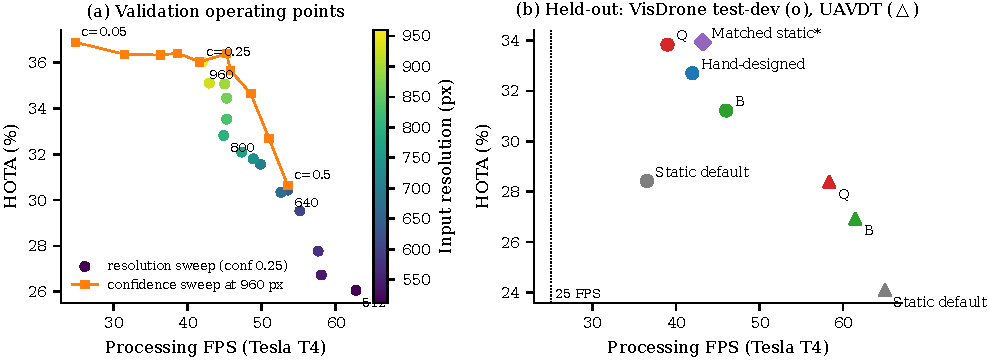
\includegraphics[width=0.95\textwidth]{figures/fig4_accuracy_runtime.pdf}
\caption{Accuracy versus processing throughput on one Tesla T4. (a) Validation operating points: resolution sweep at confidence 0.25 and confidence sweep at 960 pixels. (b) Held-out systems on VisDrone test-dev (circles) and UAVDT (triangles); the matched static anchor (diamond) was timed in a separate session. The dotted line marks 25 frames per second.}
\label{fig:runtime}
\end{figure}

\begin{table}[t]
\centering
\caption{Accuracy--throughput trade-off of the detector input resolution on VisDrone2019-MOT validation (confidence 0.25, NMS IoU 0.70, tuned tracker; T4 processing throughput and 95th-percentile per-frame latency).}
\label{tab:speed}
\small
\begin{tabular}{rrrrrrr}
\hline
Resolution & HOTA & MOTA & IDF1 & IDS & FPS & P95 latency (ms) \\
\hline
512 & 26.05 & 13.93 & 26.00 & 216 & 62.7 & 26.1 \\
576 & 27.77 & 15.67 & 29.19 & 240 & 57.6 & 29.0 \\
640 & 30.43 & 16.96 & 32.23 & 326 & 53.5 & 32.1 \\
704 & 31.56 & 17.35 & 34.26 & 322 & 49.8 & 33.6 \\
768 & 32.09 & 18.15 & 34.45 & 359 & 47.3 & 36.9 \\
832 & 33.53 & 18.92 & 37.02 & 413 & 45.3 & 37.5 \\
896 & 35.07 & 20.17 & 39.08 & 399 & 45.0 & 38.2 \\
928 & 35.10 & 20.67 & 39.70 & 416 & 42.9 & 38.6 \\
960 & 36.03 & 20.87 & 40.25 & 420 & 42.0 & 40.9 \\
\hline
\end{tabular}
\end{table}


\subsection{Resolution dominates both accuracy and cost}
In the validation sweep, raising the input resolution from 512 to 960 pixels raised HOTA from 26.05\% to 36.03\% and lowered throughput from 62.7 to 42.0 frames per second, with the 95th-percentile per-frame latency growing from 26.1 to 40.9 ms. The confidence threshold mostly moves the balance between false positives and false negatives: at 960 pixels, HOTA stayed within 36.9\% and 35.6\% for thresholds between 0.05 and 0.35 and fell to 30.6\% at 0.50, while false positives fell from 18,056 to 3,426. The very low thresholds cost throughput through the tracker (24.8 frames per second at 0.05), which is why they failed the gate. The suppression threshold had almost no effect between 0.30 and 0.55 and hurt identity switches above 0.60 (266 switches at 0.30--0.50, 467 at 0.80). The calibrated profiles lie close to the best sweep points, which is consistent with the finding that their benefit is the operating point itself.

\subsection{Held-out throughput}
All held-out systems met the gate on the whole split, and every individual test-dev sequence was processed above 25 frames per second by every system (the slowest sequence of the quality profile ran at 27.5). The balanced profile was the fastest adaptive system (46.02 frames per second on test-dev), because it spends part of the time at 512 pixels.

\subsection{Measurement variability}
Throughput measured in separate sessions on the same processor class varies more than the differences between some systems. The static anchor configuration was timed at 37.92 frames per second in the component ablation and at 44.78 in the suppression sweep, with identical tracking metrics. The full hand-designed controller was timed at 37.96, 42.09, and 43.95 frames per second in three validation runs of the same configuration. Throughput differences of a few frames per second between systems measured in different sessions, including the 2.97 frames-per-second difference between the quality profile and the hand-designed controller on test-dev, should therefore not be interpreted as algorithmic differences. The accuracy metrics are unaffected by this variability.

\section{Failure Analysis}\label{sec:failure}

\subsection{Identity switches}
The largest failure of the quality profile is identity fragmentation relative to the hand-designed controller on test-dev (123 more switches, significant). On validation the two were matched by construction (270 against 271 switches), so the constraint of Eq.~\eqref{eq:objective} did not transfer. A plausible mechanism is the tracker interaction of Sec.~\ref{sec:pipeline}: with a precision-oriented confidence threshold, boxes that briefly drop below the threshold disappear from the tracker entirely, and ByteTrack's low-score recovery cannot bridge them. The balanced profile, which optimized identity switches directly, did control them on both datasets.

\subsection{Sequences where adaptation loses}
Against the hand-designed controller, the quality profile lost on four of the 17 test-dev sequences by 0.10, 0.79, 1.87, and 4.69 HOTA points. On UAVDT, the quality profile lost to the static default on three of 20 sequences, by 1.48 to 2.29 points. The balanced profile's worst UAVDT sequence lost 12.52 points against the default, with false negatives rising from 3,477 to 4,256: its fixed confidence threshold of 0.40 removes true detections that the default's 0.25 keeps. A fixed precision-oriented threshold is therefore a risk under a domain shift that lowers detector confidence.

\subsection{Scenes outside the detector's reach}
Three UAVDT sequences had HOTA below 0.5\% for every system, and in one of them every system missed all 75,412 ground-truth boxes. No operating point recovers objects that the detector does not produce at any threshold. These sequences were kept in all aggregates. Their cause (detector coverage, class definitions, or annotation conventions) was not diagnosed within the frozen protocol, so the paper does not attribute them.

\subsection{Why switching did not help}
The calibrated search removed the conditions under which switching helps. The hand-designed controller switches between resolutions on the steep part of the accuracy--resolution curve (640--832 pixels), where a scene-dependent increase buys real recall. The calibrated profile starts from the top of that curve; above 928 pixels, the sweep gains only 0.92 HOTA points up to 960 pixels, so downward switches cost accuracy and upward switches are impossible. With seven validation sequences and a throughput gate that 960 pixels already meets, the search's best strategy was to stay high. Scene-driven switching should therefore be expected to pay off when the throughput budget does not admit the best static operating point, which is the regime of the hand-designed controller and of lower-power processors.

\IfFileExists{figures/fig7_scene_examples.pdf}{%
\begin{figure}[t]
\centering
\includegraphics[width=0.95\textwidth]{figures/fig7_scene_examples.pdf}
\caption{First frames of VisDrone validation sequences with their raw image cues (mean gray level, Laplacian variance, mean gradient magnitude) and the position of each value relative to the quartiles of the calibration set. Calibrated ranks, not raw values, enter the scene complexity index.}
\label{fig:scenes}
\end{figure}
Figure~\ref{fig:scenes} illustrates the range of validation scenes and the cue values the controller reads from them.}{}

\section{Limitations}\label{sec:limits}
The study has the following limitations.
\begin{enumerate}
\item \emph{One detector and one tracker.} All results use a COCO-pretrained YOLOv8n and ByteTrack. The absolute accuracy is limited by the absence of aerial fine-tuning, and the conclusions about which parameters matter may differ for detectors with different confidence calibration or for trackers with appearance models.
\item \emph{Research evaluation protocol.} The VisDrone evaluation is class-agnostic and uses a custom ground-truth filter; it is not the official VisDrone protocol, and the numbers are not comparable with published leaderboard results.
\item \emph{Processor and timing.} Throughput was measured on a Tesla T4, a data-center graphics processor, not on an embedded flight computer, and excludes JPEG decoding. With decoding, throughput fell below the gate. No flight test was performed. Between-session timing variability is several frames per second.
\item \emph{Small validation set.} All design decisions used seven validation sequences. The weakly identified blur and low-light weights, and the transfer failure of the identity-switch constraint, are consistent with that size.
\item \emph{Post hoc attribution.} The matched static anchor was evaluated after the freeze and timed in another session. It is the correct control for the attribution question, but it was not a preregistered competitor.
\item \emph{Statistical resolution.} Intervals come from 5,000 resamples of 17 or 20 sequences; differences of a few tenths of a HOTA point are below the resolution of the test.
\item \emph{Provenance.} The notebook cell that produced the hand-designed controller's component ablation was not recovered, although its outputs and the evaluation chain are preserved; the quality-profile test worker resumed from sequence checkpoints; and the balanced profile's first test attempt was interrupted before any result was saved. Early exploratory robustness experiments (noise, compression, frame dropping) have no canonical record and are not reported.
\end{enumerate}

\section{Conclusions}\label{sec:conclusions}
This paper studied causal, training-free control of the detector operating point for multi-object tracking in unmanned aerial vehicle video. A scene complexity index built from five calibrated cues drove the confidence threshold, the suppression threshold, and the input resolution of a fixed detector feeding ByteTrack, and all parameters were selected on validation data and frozen before a locked held-out test.

The validation-selected quality profile improved held-out HOTA over a static default by 5.41 points on VisDrone test-dev and by 4.30 points on UAVDT without retuning, and it improved over a hand-designed adaptive controller by 1.14 points while producing significantly more identity switches. A matched static configuration at the profile's typical operating point reached the same held-out accuracy, so the improvement is due to the validation-calibrated operating point and tracker profile rather than to frame-to-frame switching. The balanced profile provided a reproducible trade-off with fewer identity switches, fewer false positives, and higher throughput on VisDrone.

The ablations bound the value of scene-driven switching: it added accuracy for the hand-designed controller, whose resolution range lies on the steep part of the accuracy--resolution curve, and it added none for the calibrated controller, whose search placed it at the top of that curve within the available throughput budget. For aerial tracking systems, the practical conclusion is that the detector operating point and the tracker profile should be calibrated on representative aerial validation data before any adaptive mechanism is added, and that adaptation should be evaluated against a matched static operating point.

\section*{Acknowledgments}
The author thanks the maintainers of the VisDrone and UAVDT benchmarks and of the TrackEval library.

\bibliography{references}

\end{document}
